\documentclass[UTF8,fontset=none,12pt]{ctexart}

\setCJKmainfont{Songti SC}
\setCJKsansfont{PingFang SC}
\setCJKmonofont{Songti SC}

\usepackage[a4paper,margin=2.35cm]{geometry}
\usepackage{amsmath,amssymb,amsthm,mathtools,bm}
\usepackage{graphicx}
\usepackage{float}
\usepackage{booktabs}
\usepackage{enumitem}
\usepackage[hidelinks]{hyperref}

\newcommand{\C}{\mathbb{C}}
\newcommand{\R}{\mathbb{R}}
\newcommand{\rank}{\operatorname{rank}}
\newcommand{\sign}{\operatorname{sign}}

\title{数值线性代数\quad 第 10 讲：Householder 三角化}
\author{Lloyd N. Trefethen、David Bau III\quad 中文阅读版}
\date{}

\begin{document}
\maketitle
\pagestyle{plain}

计算 QR 分解的另一种主要方法是 Householder 三角化.它在数值上比 Gram--Schmidt 正交化更稳定，不过不像后者那样适合作为迭代方法的基础. Householder 算法通过一系列酉矩阵运算把矩阵变成三角形，因此也可以看成\textbf{正交三角化}.

\section*{Householder 与 Gram--Schmidt}

在第 8 讲中，我们看到 Gram--Schmidt 迭代在 $A$ 的右侧依次乘上一些初等三角矩阵 $R_k$，从而得到
\begin{equation}
    A R_1R_2\cdots R_n=\widehat Q,
    \qquad
    R_1R_2\cdots R_n=\widehat R^{-1},
\end{equation}
其中 $\widehat Q$ 的列是标准正交的.因此
\[
    \widehat R=R_n^{-1}\cdots R_2^{-1}R_1^{-1}
\]
仍是上三角矩阵，于是 $A=\widehat Q\widehat R$ 是 $A$ 的约化 QR 分解.

相比之下，Householder 方法在 $A$ 的左侧依次乘上初等酉矩阵 $Q_k$，使得
\begin{equation}
    Q_n\cdots Q_2Q_1A=R,
    \qquad
    Q^*=Q_n\cdots Q_2Q_1,
\end{equation}
其中 $R$ 是上三角矩阵.乘积
\[
    Q=Q_1^*Q_2^*\cdots Q_n^*
\]
也是酉矩阵，因此 $A=QR$ 是一个\textbf{完整} QR 分解.

所以，这两种方法可以概括为：
\[
\begin{array}{ll}
\text{Gram--Schmidt:}&\text{三角正交化（triangular orthogonalization）},\\
\text{Householder:}&\text{正交三角化（orthogonal triangularization）}.
\end{array}
\]

\section*{通过引入零元素进行三角化}

Householder 方法的核心思想最初由 Alston Householder 于 1958 年提出.它巧妙地设计酉矩阵 $Q_k$，使
\[
    Q_n\cdots Q_2Q_1A
\]
成为上三角矩阵.

矩阵 $Q_k$ 的作用，是在第 $k$ 列主对角线下方引入零元素，同时保留此前已经引入的所有零元素.例如，对 $5\times3$ 矩阵，依次应用三个运算 $Q_k$，结构如下.图中 $\times$ 表示不一定为零的元素；黑体元素表示刚刚被改变的元素；空白位置表示零.

\begin{figure}[H]
    \centering
    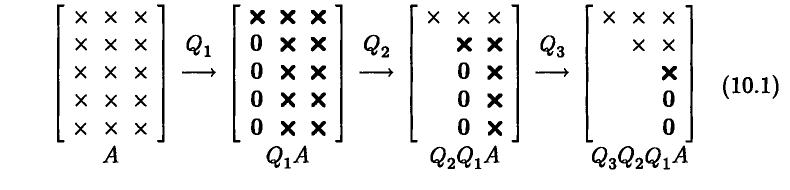
\includegraphics[width=0.98\linewidth]{../assets/figure-10-1-zero-introduction.png}
    \caption{Householder 三角化通过逐列引入零元素.}
    \label{fig:10-1-zero-introduction}
\end{figure}

首先，$Q_1$ 作用于第 $1,\ldots,5$ 行，在位置 $(2,1),(3,1),(4,1),(5,1)$ 引入零元素.接着，$Q_2$ 作用于第 $2,\ldots,5$ 行，在位置 $(3,2),(4,2),(5,2)$ 引入零元素，同时不会破坏 $Q_1$ 引入的零元素.最后，$Q_3$ 作用于第 $3,\ldots,5$ 行，在位置 $(4,3),(5,3)$ 引入零元素，也不会破坏前面已经引入的零元素.

一般地，$Q_k$ 作用于第 $k,\ldots,m$ 行.在第 $k$ 步开始时，这些行的前 $k-1$ 列已经形成一个零块. $Q_k$ 对这些行做线性组合，而零元素的线性组合仍然为零.经过 $n$ 步，主对角线下方的所有元素都被消去，$Q_n\cdots Q_2Q_1A=R$ 成为上三角矩阵.

\section*{Householder 反射器}

如何构造能够实现上述零元素结构的酉矩阵 $Q_k$？标准做法是把每个 $Q_k$ 取为
\begin{equation}
    Q_k=
    \begin{bmatrix}
        I&0\\
        0&F
    \end{bmatrix},
    \tag{10.2}
\end{equation}
其中 $I$ 是 $(k-1)\times(k-1)$ 单位矩阵，$F$ 是 $(m-k+1)\times(m-k+1)$ 的酉矩阵.矩阵 $F$ 的乘法必须在第 $k$ 列中引入所需的零元素. Householder 算法取 $F$ 为一种称为 Householder 反射器的特殊矩阵.

假设在第 $k$ 步开始时，第 $k$ 列的第 $k,\ldots,m$ 个元素组成向量
\[
    x\in\C^{m-k+1}.
\]
为了在第 $k$ 列引入正确的零元素，Householder 反射器 $F$ 应实现如下映射：
\begin{equation}
    x=
    \begin{bmatrix}
        \times\\
        \times\\
        \vdots\\
        \times
    \end{bmatrix}
    \ \xrightarrow{\quad F\quad}\
    Fx=
    \begin{bmatrix}
        \|x\|_2\\
        0\\
        \vdots\\
        0
    \end{bmatrix}
    =\|x\|_2e_1.
    \tag{10.3}
\end{equation}
稍后我们会在这个想法上加入一个 $\pm$ 号.

图~\ref{fig:10-1-reflection} 描绘了这种构造.反射器 $F$ 把空间 $\C^{m-k+1}$ 关于与
\[
    v=\|x\|_2e_1-x
\]
正交的超平面 $H$ 进行反射.超平面是二维平面在高维空间中的推广：它可以是四维空间中的三维子空间，也可以是五维空间中的四维子空间，依此类推.一般而言，超平面可以刻画为与某个非零固定向量正交的全部点组成的集合.在图~\ref{fig:10-1-reflection} 中，这个固定向量就是 $v=\|x\|_2e_1-x$；虚线可以理解为从“侧面”观察超平面 $H$ 得到的示意.

\begin{figure}[H]
    \centering
    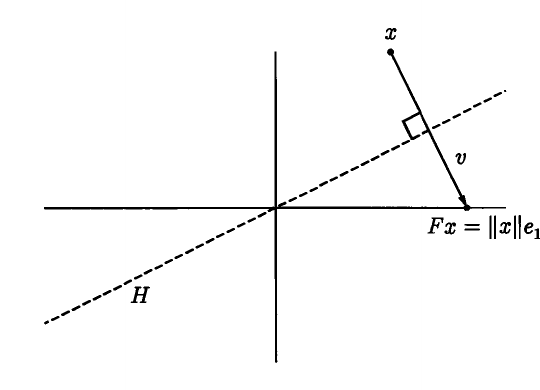
\includegraphics[width=0.72\linewidth]{../assets/figure-10-1-reflection.png}
    \caption{Householder 反射.}
    \label{fig:10-1-reflection}
\end{figure}

施加反射后，超平面 $H$ 一侧的每个点都会被映到另一侧的镜像点.特别地，$x$ 被映到 $\|x\|_2e_1$.反射公式可以这样推导.第 6 讲的式 (6.11) 告诉我们，对任意 $y\in\C^m$，向量
\begin{equation}
    Py=
    \left(I-\frac{vv^*}{v^*v}\right)y
    =y-v\left(\frac{v^*y}{v^*v}\right)
\end{equation}
是 $y$ 在超平面 $H$ 上的正交投影.如果要把 $y$ 关于 $H$ 反射，就不能停在投影点；而要沿同一方向再走同样的距离.因此
\begin{equation}
    Fy=
    \left(I-2\frac{vv^*}{v^*v}\right)y
    =y-2v\left(\frac{v^*y}{v^*v}\right).
\end{equation}
于是反射矩阵为
\begin{equation}
    F=I-2\frac{vv^*}{v^*v}.
    \tag{10.4}
\end{equation}
注意，投影矩阵 $P$ 的秩为 $m-1$，而反射器 $F$ 满秩且酉；二者的公式只差一个因子 2.

\section*{两个反射器中更好的一个}

式 (10.3) 和图~\ref{fig:10-1-reflection} 把问题简化了.事实上，有许多 Householder 反射都能引入所需的零元素.向量 $x$ 可以被反射到
\[
    z\|x\|_2e_1,\qquad |z|=1.
\]
在复数情形中，这些可能的反射形成一个圆；即使在实数情形中，也有两个选择，分别对应关于不同超平面 $H^+$ 与 $H^-$ 的反射，如图~\ref{fig:10-2-reflections} 所示.

\begin{figure}[H]
    \centering
    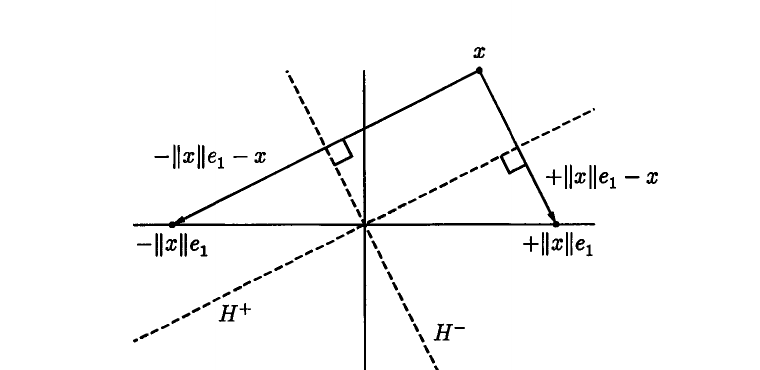
\includegraphics[width=0.78\linewidth]{../assets/figure-10-2-reflections.png}
    \caption{两个可能的反射.为了数值稳定，应选择使 $x$ 移动距离更大的那个.}
    \label{fig:10-2-reflections}
\end{figure}

从数学上说，选择哪一个符号都没有问题.但是，数值稳定性的目标---也就是对舍入误差不敏感---要求我们固定采用其中一个选择.为了稳定，最好把 $x$ 反射到不太接近 $x$ 本身的向量 $z\|x\|_2e_1$.为此，取
\[
    z=-\sign(x_1),
\]
其中 $x_1$ 是 $x$ 的第一个分量.此时反射向量为
\[
    v=-\sign(x_1)\|x\|_2e_1-x.
\]
把整体因子 $-1$ 消去，得到更方便的表达式
\begin{equation}
    v=\sign(x_1)\|x\|_2e_1+x.
    \tag{10.5}
\end{equation}
为了使这成为完整的规定，可以约定 $x_1=0$ 时 $\sign(x_1)=1$.

这个符号选择为何影响稳定性并不难看出.假设图~\ref{fig:10-2-reflections} 中 $H^+$ 与 $e_1$ 轴的夹角非常小.那么
\[
    v=\|x\|_2e_1-x
\]
会比 $x$ 或 $\|x\|_2e_1$ 小得多.计算 $v$ 时要把两个很接近的量相减，因此容易发生消去误差.采用式 (10.5) 中的符号，可以保证 $\|v\|_2$ 不会小于 $\|x\|_2$，从而避免这种效应.

\section*{算法}

现在给出完整的 Householder 算法.先介绍一种新的 MATLAB 风格记号.若 $A$ 是一个矩阵，记
\[
    A_{i:i',\,j:j'}
\]
为 $A$ 的子矩阵：其左上角为 $a_{i,j}$，右下角为 $a_{i',j'}$，尺寸为 $(i'-i+1)\times(j'-j+1)$.当子矩阵退化为单行或单列的子向量时，分别写作
\[
    A_{i,\,j:j'}\quad\text{或}\quad A_{i:i',\,j}.
\]

下面的算法计算 $m\times n$ 矩阵 $A$ 的 QR 分解中的 $R$ 因子，其中 $m\ge n$；算法直接在 $A$ 原位置上写回结果.同时，它把 $n$ 个反射向量 $v_1,\ldots,v_n$ 保存下来，以便后续使用.

\subsection*{算法 10.1：Householder QR 分解}

\begin{verbatim}
for k = 1 to n
    x = A(k:m,k)
    v_k = sign(x_1)||x||_2 e_1 + x
    v_k = v_k/||v_k||_2
    A(k:m,k:n) = A(k:m,k:n) - 2v_k(v_k^*A(k:m,k:n))
\end{verbatim}

\section*{应用或构造 $Q$}

算法 10.1 完成后，$A$ 已经被化为上三角形式；这就是 QR 分解 $A=QR$ 中的 $R$.不过，酉矩阵 $Q$ 尚未构造出来，与约化 QR 分解对应的 $n$ 列子矩阵 $\widehat Q$ 也尚未构造.这是有意的：显式构造 $Q$ 或 $\widehat Q$ 需要额外工作，而许多应用可以直接使用
\begin{equation}
    Q^*=Q_n\cdots Q_2Q_1
    \tag{10.6}
\end{equation}
或它的共轭
\begin{equation}
    Q=Q_1Q_2\cdots Q_n.
    \tag{10.7}
\end{equation}
这里没有漏写星号；回忆一下，每个 $Q_j$ 都是 Hermitian 矩阵.

例如，第 7 讲说明了如何通过 QR 分解求解方程组 $Ax=b$.在这个过程中，使用 $Q$ 的唯一地方是计算 $Q^*b$.根据式 (10.6)，可以对 $b$ 依次施加 $n$ 个运算来计算 $Q^*b$；这些运算与把 $A$ 化为三角矩阵时所做的运算完全相同.

\subsection*{算法 10.2：隐式计算 $Q^*b$}

\begin{verbatim}
for k = 1 to n
    b(k:m) = b(k:m) - 2v_k(v_k^*b(k:m))
\end{verbatim}

类似地，计算 $Qx$ 只需按相反顺序执行同样的过程.

\subsection*{算法 10.3：隐式计算 $Qx$}

\begin{verbatim}
for k = n downto 1
    x(k:m) = x(k:m) - 2v_k(v_k^*x(k:m))
\end{verbatim}

上述两个算法的工作量都是 $O(mn)$，而不是算法 10.1 的 $O(mn^2)$（见下文）.

当然，有时我们确实希望显式构造矩阵 $Q$.一种办法是使用算法 10.3，分别计算
\[
    Qe_1,\ Qe_2,\ \ldots,\ Qe_m
\]
作为 $Q$ 的各列.另一种办法是使用算法 10.2 构造 $Q^*$，然后取共轭转置.还可以在每一步都取共轭，而不是最后才处理整个乘积：按照式 (10.7) 的启发，计算
\[
    e_1^*Q,\ e_2^*Q,\ \ldots,\ e_m^*Q
\]
作为 $Q$ 的各行.在这些方法中，最好的通常是第一种，即基于算法 10.3 的方法.原因是它从涉及 $Q_n,Q_{n-1},\ldots$ 的运算开始，而这些运算只会修改所作用向量的一小部分；利用这种稀疏性可以加速.

如果只需要 $\widehat Q$ 而不需要完整的 $Q$，只需计算前 $n$ 列
\[
    Qe_1,\ Qe_2,\ \ldots,\ Qe_n.
\]

\section*{运算量}

算法 10.1 的工作量主要由内层更新决定：
\begin{equation}
    A_{k:m,j}
    =
    A_{k:m,j}-2v_k\bigl(v_k^*A_{k:m,j}\bigr).
    \tag{10.8}
\end{equation}
若向量长度为 $\ell=m-k+1$，这次计算需要 $4\ell-1\approx4\ell$ 次标量运算：减法 1 次，标量乘法 1 次，内积需要 $2\ell-1$ 次.也就是说，每个被处理的矩阵元素约对应 4 次浮点运算.

像第 8 讲那样，可以用几何方法把每个元素的 4 次 flop 加总.外层循环的每个后续步骤都作用于更少的行，因为第 $k$ 步不会改变第 $1,\ldots,k-1$ 行.同时，每一步也作用于更少的列，因为被处理行的第 $1,\ldots,k-1$ 列已经是零，会被跳过.因此，一个外层步骤的工作量可以表示为下面立体图的一个横层.

\begin{figure}[H]
    \centering
    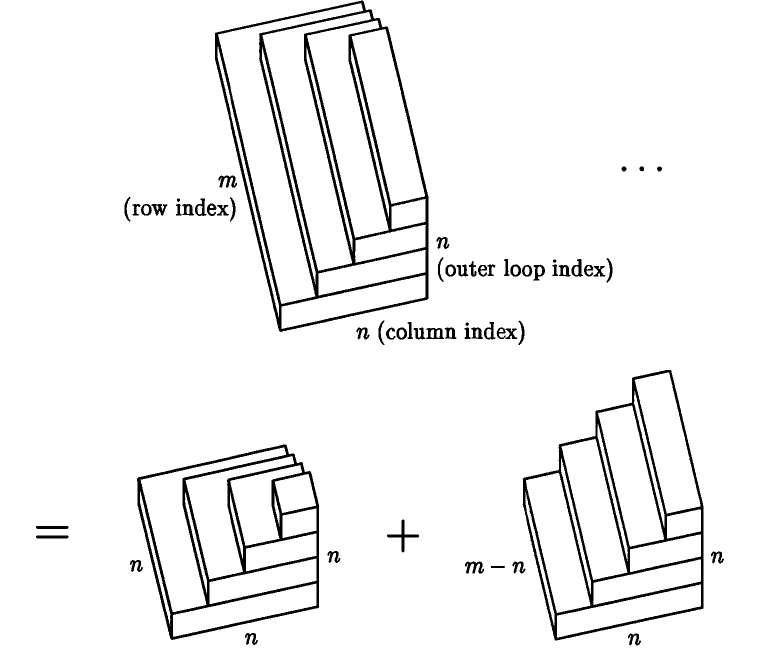
\includegraphics[width=0.83\linewidth]{../assets/figure-10-operation-count.png}
    \caption{Householder 正交化运算量的几何图示.上图表示每个外层步骤对应的一个横层，下方把这个立体分成“之”字形部分和阶梯形部分.}
    \label{fig:10-operation-count}
\end{figure}

总运算次数等于该立体体积的 4 倍.为了从图形上确定体积，可以把立体分成两部分.左侧立体呈锯齿形；当 $n\to\infty$ 时趋近于一个体积为 $\frac13n^3$ 的棱锥.右侧立体呈阶梯形；当 $m,n\to\infty$ 时趋近于一个体积为
\[
    \frac12(m-n)n^2
\]
的棱柱.合并两部分，体积为
\[
    \sim \frac12mn^2-\frac16n^3.
\]
再乘以每单位体积 4 次 flop，得到
\begin{equation}
    \text{Householder 正交化的工作量}
    \sim 2mn^2-\frac23n^3\ \text{flops}.
    \tag{10.9}
\end{equation}

\section*{习题}

\begin{enumerate}[label=\textbf{10.\arabic*}]
    \item 确定一个 Householder 反射器的：(a) 特征值；(b) 行列式；(c) 奇异值.对于特征值，请同时给出几何论证和代数证明.

    \item
    \begin{enumerate}[label=(\alph*)]
        \item 编写 MATLAB 函数 \texttt{[W,R] = house(A)}.它使用 Householder 反射，为 $m\times n$ 矩阵 $A$（$m\ge n$）的完整 QR 分解 $A=QR$ 计算一个隐式表示.输出变量是 $W\in\C^{m\times n}$ 的下三角矩阵，其列是定义各次 Householder 反射的向量 $v_k$，以及三角矩阵 $R\in\C^{n\times n}$.
        \item 编写 MATLAB 函数 \texttt{Q = formQ(W)}.它以 \texttt{house} 产生的矩阵 $W$ 为输入，生成相应的 $m\times m$ 正交矩阵 $Q$.
    \end{enumerate}

    \item 令
    \[
        Z=
        \begin{bmatrix}
            1&2&3\\
            4&5&6\\
            7&8&7\\
            4&2&3\\
            4&2&2
        \end{bmatrix}.
    \]
    在 MATLAB 中计算 $Z$ 的三种约化 QR 分解：使用习题 8.2 的 Gram--Schmidt 程序 \texttt{mgs}；使用习题 10.2 的 Householder 程序 \texttt{house} 和 \texttt{formQ}；以及 MATLAB 内置命令 \texttt{[Q,R] = qr(Z,0)}.比较这三种结果，并说明你观察到的差异.

    \item 考虑两个 $2\times2$ 正交矩阵
    \begin{equation}
        F=
        \begin{bmatrix}
            -c&s\\
            s&c
        \end{bmatrix},
        \qquad
        J=
        \begin{bmatrix}
            c&s\\
            -s&c
        \end{bmatrix},
        \qquad
        s=\sin\theta,\quad c=\cos\theta.
        \tag{10.10}
    \end{equation}
    第一个矩阵满足 $\det F=-1$，是一个反射器---二维 Householder 反射器的特殊情形.第二个矩阵满足 $\det J=1$，执行的是旋转而不是反射；这样的矩阵称为 Givens 旋转.
    \begin{enumerate}[label=(\alph*)]
        \item 准确描述左乘 $F$ 和 $J$ 对平面 $\R^2$ 的几何作用.例如，$J$ 把平面旋转 $\theta$ 角，但旋转是顺时针还是逆时针？
        \item 描述一种基于 Givens 旋转的 QR 分解算法，使其对应于算法 10.1，但用 Givens 旋转代替 Householder 反射.
        \item 证明你的算法每个被处理元素需要 6 次 flop，而不是 4 次，因此渐近运算量比式 (10.9) 大 50\%.
    \end{enumerate}
\end{enumerate}

\end{document}
